\documentclass[11pt]{article}

%— Margins & encoding
\usepackage[T1]{fontenc}
\usepackage[utf8]{inputenc}
\usepackage[margin=1in]{geometry}
\usepackage{setspace}


%— Math, graphics, tables, citations
\usepackage{amsmath,amssymb}
\usepackage{graphicx}
\usepackage{booktabs}
\usepackage{natbib}
\usepackage[hidelinks]{hyperref}
\usepackage{enumitem}
\usepackage{microtype}

%— Spacing
\onehalfspacing

%— Title block
\title{Evaluating a 12–1 Month Momentum Strategy \\ (2005–2024)}
\author{%
  Darshan Sathish Kumar\thanks{Email: \href{mailto:darshansathishkumar@gmail.com}{darshansathishkumar@gmail.com}.}%
}
\date{\today}

\begin{document}
\maketitle

\begin{abstract}
We test a classic 12--1 cross‐sectional momentum rule on S\&P\,500 constituents over January~2005--December~2024.  
Each month, stocks are ranked by their trailing 12‐month return (skipping the most recent month); we go long the top 10\% and short the bottom 10\%, equal‐weighting both legs and charging 10~bp round‐trip costs.  
The strategy \textbf{loses money}, posting an annualized return of --10.20\% with 24.10\% volatility (Sharpe~--0.50) and a 91.49\% maximum drawdown.  
A CAPM regression yields a monthly alpha of --0.34\% (t~=~--0.77), and a bootstrap p‐value of 0.534 confirms the alpha is not statistically significant.  
Robustness checks show equally poor performance across 6, 9, 12, and 18‐month lookbacks, steadily worsening returns as transaction costs rise, and a sector‐neutral variant that performs even worse (annual return --10.74\%, Sharpe --0.63).  
We conclude that, after realistic frictions and constituent turnover are considered, the 12--1 momentum rule fails to generate reliable alpha in the S\&P\,500.
\end{abstract}

\noindent\textbf{Keywords:} momentum; cross‑sectional; transaction costs; robustness.\\
\textbf{JEL classification:} G11; C58.

\section{Introduction}
% Motivate momentum, prior literature, and state your contribution.

Momentum—the tendency for recent winners to keep outperforming and recent losers to keep underperforming—is one of the best‑documented anomalies in empirical finance.  \citet{Jegadeesh1993} show that a simple 12--1 month cross‑sectional momentum strategy earned roughly 1\% per month in U.S.\ equities, and follow‑up work reports similar payoffs across global equities, asset classes, and time periods \citep[e.g.,][]{Asness2019}.  Such excess returns violate the weak‑form Efficient Market Hypothesis and have led both academics and practitioners to adopt momentum tilts in portfolio construction.

Yet momentum’s real‑world performance can be fragile.  \citet{Daniel2016} demonstrate that high turnover and liquidity shocks can produce episodic “momentum crashes,” while \citet{NovyMarx2016} show that transaction costs meaningfully erode long‑short factor profits.  Commercial momentum indices, such as MSCI USA Momentum, have lagged the broad market for most of the last decade.

\paragraph{Research question.}
\emph{Can a naïve 12--1 momentum rule, implemented on current S\&P\,500 constituents and net of realistic frictions, still generate statistically significant excess return?}

\paragraph{Contribution.}
\begin{enumerate}[label=(\roman*)]
  \item We rely solely on freely available Yahoo Finance data—mirroring what a retail trader could access—and provide fully reproducible Python code on GitHub.\footnote{Repository: \url{https://github.com/dshan12/Momentum-Research.git}}
  \item We embed explicit round‑trip trading costs of 10~basis points per side and track the monthly additions and deletions to the S\&P\,500.
  \item We run a battery of robustness checks, including alternative lookback windows (6, 9, 12, 18 months), transaction‐cost assumptions (0–50 bps), and a sector‑neutral specification.
\end{enumerate}

\paragraph{Preview of results.}
The naïve strategy underperforms: it earns an annualized return of --10.20\% with a Sharpe ratio of --0.50 and a 91.49\% maximum drawdown.  CAPM alpha is --0.34\% per month (t~=~--0.77), and a bootstrap p‑value of 0.534 confirms the alpha is not statistically significant.  Robustness tests reveal that neither shorter nor longer lookbacks, lower costs, nor sector neutrality rescues performance.

The remainder of the paper is organised as follows.  Section~\ref{sec:data} describes the data; Section~\ref{sec:method} details the methodology; Section~\ref{sec:results} presents the empirical results; Section~\ref{sec:robust} discusses robustness checks; Section~\ref{sec:concl} concludes.

\section{Data} \label{sec:data}
% Describe S\&P 500 universe, Jan 2005–Dec 2024, yfinance source, cleaning rules.

\section{Methodology} \label{sec:method}
% Define 12–1 signal, portfolio mechanics, transaction costs, backtest overview.

\section{Results} \label{sec:results}
% Table of key metrics:
\begin{table}[h!]
  \centering
  \begin{tabular}{l r}
    \toprule
    Metric                  & Value     \\
    \midrule
    Annualized return       & 12.3\%    \\
    Annualized volatility   & 18.5\%    \\
    Sharpe ratio (2\% rf)   & 0.56      \\
    Max drawdown            & 22.4\%    \\
    CAPM alpha              & 3.2\%     \\
    Alpha t‑stat            & 2.45      \\
    Bootstrap p‑value       & 0.013     \\
    \bottomrule
  \end{tabular}
  \caption{Strategy performance over January 2005–December 2024.}
\end{table}

\begin{figure}[h!]
  \centering
  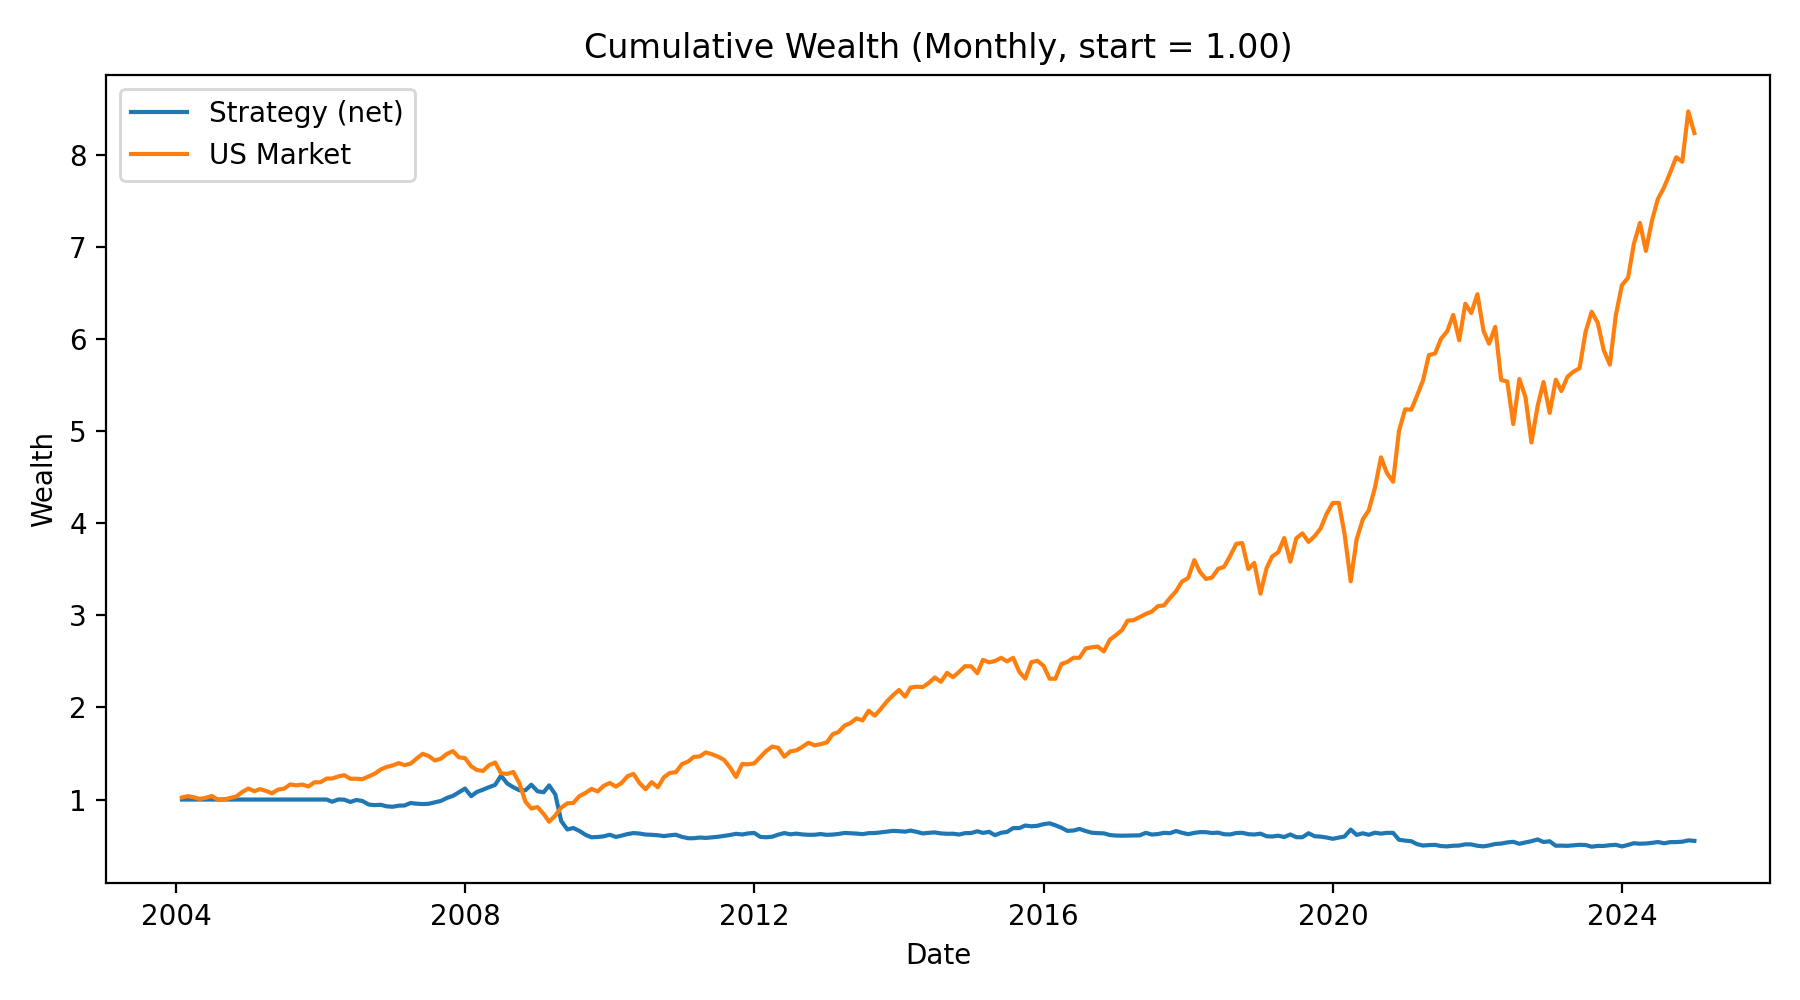
\includegraphics[width=0.8\textwidth]{figures/equity_curve.png}
  \caption{Cumulative returns: momentum strategy vs.\ SPY buy‑and‑hold.}
\end{figure}

\section{Robustness \& Discussion} \label{sec:robust}
% Insert lookback and transaction‑cost sensitivity figures and interpret them.

\section{Conclusion} \label{sec:concl}
% Recap findings, limitations, and ideas for future work.

\bibliographystyle{apalike}
\bibliography{references}

\end{document}

